In this system the ds-server simulates job submissions and job executions by servers, whilst the client handles the job scheduling logic. First ds-server needs to open a socket for the client to connect to (defaulting to localhost and port 50000), and then the client must connect and authenticate before any scheduling of jobs can begin.\\

\vspace{.2cm}
For stage 1 of this project, the client must implement the Largest Round-Robin (LRR) scheduling algorithm. After receiving a job, the client must decide which server it needs to be scheduled to. In LRR, the server chosen is the one with the most CPU cores total. If there are multiple equal servers, then the client needs to pick the first one that is provided. \\

\vspace{.2cm}
The flow of communication between the two whilst using LRR is outlined in the flowchart below.
\begin{center}
    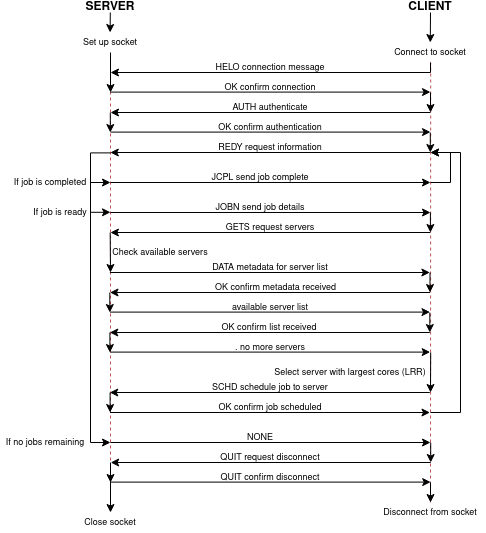
\includegraphics[scale=0.7]{Communication Flowchart.png}
\end{center}

